\begin{appendices}
\chapter{External Material}
External libraries and software used:
\begin{itemize}
	\item OpenGL
	\item Qt 5.3.1 (QtOpenGL and QtNetwork module)
	\item NetworkX (Python module)
	\item OpenDaylight 0.5.0 SDN controller
	\item Open vSwitch virtual switches
	\item Mininet virtual network simulator
	\item Wireshark network packet analyser
\end{itemize}

The load balancer code was based on code found in: \url{https://github.com/nayanseth/sdn-loadbalancing}. The code was improved by allowing for multiple traffic flows to be load balanced.

\chapter{Ethical Issues Addressed}
This project does not have any ethical issues involved since there are no human participants. Also no private or personal data was used in the process.

\chapter{User Manual}

GitHub repository at: \url{http://github.com/kvcruzat/cloudgaming/}

\section{Cloud Gaming System}

In order for the cloud gaming system to run, an environment with the following software/libraries is needed:
\begin{itemize}
	\item C++ and g++ compiler
	\item OpenGL
	\item Qt 5.3.1 or above
\end{itemize}

\subsection{Game Server}

The game folder is located in the GitHub repository in the path:
\newline
\path{cloudgaming/Implementation/game/}
\newline
\par
To compile and execute the game a \textit{make.sh} script is included in the folder for compilation and can be run with the following commands:
\begin{verbatim}
	$ sh make.sh
	$ ./game
\end{verbatim}

\subsection{Client Program}

The client program can be run locally on the same machine or on a different machine on the same network. The client folder is located in the current path:
\newline
\path{cloudgaming/Implementation/client/}
\newline
\par
To compile and execute the game a \textit{make.sh} script is included in the folder for compilation. To execute the client, IP address or host name and port number needs to be supplied as arguments. The IP address and port number is printed out on the terminal where the game server is executed. Here are example commands
\begin{verbatim}
	$ sh make.sh
	$ ./client comp-pc3085 4871
\end{verbatim}

\section{Networking}
In order for the SDN networking to run, an environment with the following software/libraries is needed:

\begin{itemize}
	\item Java 8
	\item Python 2.7.6 or above
\end{itemize}
 
\subsection{Mininet Virtual Network}
To install Mininet the following commands can be used:
\begin{verbatim}
	$ git clone git://github.com/mininet/mininet
	$ $ git checkout -b 2.2.1
	$ ./util/install.sh -a
\end{verbatim}
To run the virtual network with mininet the topology is located in the path:
\path{cloudgaming/Implementation/networking/}
To execute Mininet with the \textit{fatcloudtopo.py} topology, OpenDaylight needs to be running in another terminal (instructions in section C.2.3) then use the following command:
\begin{verbatim}
	$ sudo mn --controller=remote,ip=127.0.0.1 --custom fatcloudtopo.py 
	--topo cloudtopo --link tc
\end{verbatim}

\subsection{Open vSwitch}
To install Open vSwitch, the following installation instructions can be used:
\newline
\url{http://dannykim.me/danny/openflow/57620}
\newline
\par
The following commands are used to start Open vSwitch:
\begin{verbatim}
	$ sudo ovsdb-server --remote=punix:/usr/local/var/run/openvswitch/db.sock 
	--remote=db:Open_vSwitch,Open_vSwitch,manager_options 
	--private-key=db:Open_vSwitch,SSL,private_key 
	--certificate=db:Open_vSwitch,SSL,certificate 
	--bootstrap-ca-cert=db:Open_vSwitch,SSL,ca_cert --pidfile --detach
	$ sudo ovs-vsctl --no-wait init
	$ sudo ovs-vswitchd --pidfile --detach
\end{verbatim}

\subsection{OpenDaylight SDN Controller}
The controller can be downloaded from the following URL:
\newline
\url{https://nexus.opendaylight.org/content/repositories/opendaylight.snapshot/org/opendaylight/integration/distribution-karaf/0.5.0-SNAPSHOT/}
\newline
\par
To run the controller, Open vSwitch needs to be running (instructions in section C.2.2). The controller can be run with the following commands:
\begin{verbatim}
	$ cd distribution-karaf-0.5.0-SNAPSHOT
	$ ./bin/karaf
\end{verbatim}
In order for the controller to function correctly for this project, a few features needs to be installed. The following command needs to be executed in the controllers command line interface:
\begin{verbatim}
	<opendaylight-user@root> feature:install odl-dlux-all odl-restconf-all 
	odl-l2switch-all
\end{verbatim}
The OpenDaylight web GUI can be accessed using the following link in a browser while the controller is running:
\url{http://localhost:8181/index.html}

\subsection{Load Balancer}
To run the load balancer tests, the SDN controller (section C.2.3) needs to be running in the background and the fat tree topology running with Mininet (section C.2.1). In Mininet CLI ping all hosts (Figure \ref{fig:pingall}) and connect to hosts where traffic will be sent and received using the example following commands:
\begin{verbatim}
	mininet> pingall
	mininet> xterm h1 h2 h4 h5
\end{verbatim}
iPerf traffic simulation can be run by setting destination node in server mode and the source in client mode with the commands:
\begin{verbatim}
	h1 (10.0.0.1: Server mode):
	$ iperf -s -u
	h4 (10.0.0.4: Client mode):
	$ iperf -c 10.0.0.1 -u -b 50M -t 60
\end{verbatim}
Delay in the connection can then be tested with a simple ping command with 10 packets in the Mininet CLI:
\begin{verbatim}
	mininet> h1 ping -c 10 h4
\end{verbatim}
The load balancer can be run using another terminal and the path for the python script \textit{load\_balancer.py} is in:
\path{cloudgaming/Implementation/networking}
The load balancer for the connection between h1 (10.0.0.1) and h4 (10.0.0.4) can be executed as follows:
\begin{verbatim}
	$ python load_balancer.py 
	Enter Host 1
	1

	Enter Host 2
	4
\end{verbatim}
The installed flows can be deleted by running the python script \textit{deleteflows.py}
\begin{verbatim}
	$ python deleteflows.py
\end{verbatim}

\begin{figure}[h!]
 \centering
 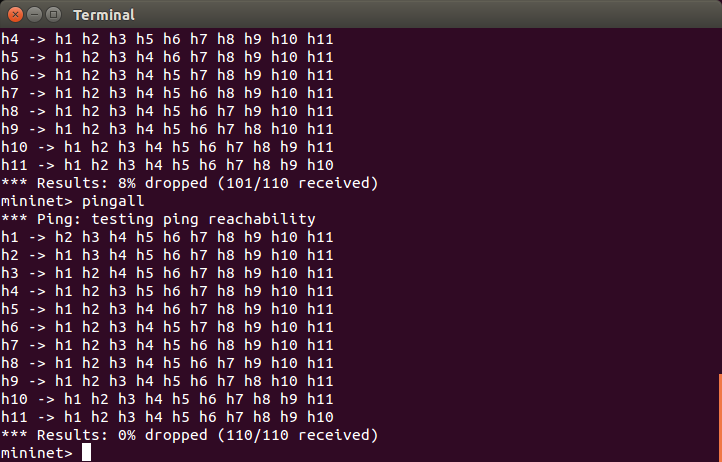
\includegraphics[width=\linewidth]{images/loadbalancing/mnpingall.png}
 \caption{Screenshot of all hosts discovering each other through pingall command}
 \label{fig:pingall}
\end{figure}


\end{appendices}